\documentclass[11pt,a4paper]{article}
\usepackage[margin=0.85in]{geometry}
\usepackage[T1]{fontenc}
\usepackage[table]{xcolor}
\usepackage{lmodern,booktabs,longtable,array,enumitem,hyperref,tikz,fancyhdr,adjustbox}
\usetikzlibrary{arrows.meta,positioning,shapes.geometric,fit}
\definecolor{navy}{HTML}{17365D}\definecolor{blue}{HTML}{3468A0}\definecolor{pale}{HTML}{E9F1FA}
\hypersetup{colorlinks=true,linkcolor=navy,urlcolor=blue}
\pagestyle{fancy}\fancyhf{}\lhead{STUDEND | Capstone Proposal}\rhead{\thepage}\renewcommand{\headrulewidth}{0.3pt}
\setlength{\headheight}{14pt}
\setlength{\parskip}{5pt}\setlength{\parindent}{0pt}\emergencystretch=3em
\newcommand{\heading}[1]{\vspace{5pt}\textcolor{navy}{\textbf{#1}}}
\tikzset{box/.style={draw=blue,rounded corners=3pt,fill=pale,align=center,minimum height=9mm,font=\small},arrow/.style={-{Stealth[length=2mm]},thick,draw=navy},actor/.style={draw=navy,ellipse,fill=pale,align=center,font=\small},entity/.style={draw=navy,rectangle,fill=pale,align=center,font=\small,minimum height=9mm}}
\begin{document}
\begin{titlepage}
\thispagestyle{empty}
\begin{center}
\vspace*{1.15cm}
{\Large\bfseries Final Capstone Project Proposal\par}
\vspace{0.30cm}
{\large Part I --- Proposal and Prototyping\par}
\vspace{1.25cm}
{\Huge\bfseries\textcolor{navy}{STUDEND}\par}
\vspace{0.45cm}
{\Large An AI-Powered University Academic Management\par}
\vspace{0.12cm}
{\Large and Intelligent Learning Assistance System\par}
\vspace{0.65cm}
{\normalsize Java Web Application with Cloud AI Integration\par}
\vspace{3.25cm}
\begin{minipage}{0.88\textwidth}
\renewcommand{\arraystretch}{1.45}
\begin{tabular}{@{}p{3.3cm}p{9.3cm}@{}}
\textbf{Prepared by} & MD. Afif Zaman \\
\textbf{Student ID} & IT-23059 \\
\textbf{Course} & Software Engineering and Project Management \\
\textbf{Submitted to} & Prof. Dr. Ziaur Rahman \\
\textbf{University} & Mawlana Bhashani Science and Technology University \\
\textbf{Proposal version} & 1.0 --- November 2026
\end{tabular}
\end{minipage}
\end{center}
\vfill
\end{titlepage}
\tableofcontents\newpage
\section{Executive Summary}
STUDEND is a proposed role-based academic management platform for universities, integrating administration, course delivery, and AI-assisted learning. The Java web application will allow university administrators to manage students, teachers, batches, and courses; teachers to upload materials and prepare assignments; and students to access course information and an intelligent study assistant. A cloud-based language model API will support document summarization, material-grounded question answering, and teacher-reviewed assignment drafting. The project will use an iterative and incremental process and deliver an initial working prototype followed by tested enhancements.
\section{Problem Statement and Motivation}
Academic information is often distributed across spreadsheets, messaging applications, shared folders, and separate learning tools. This creates duplicate data entry, inconsistent access to course materials, difficulty tracking enrollment, and additional work for teachers preparing learning activities. Generic AI tools may also answer without access to the specific lecture material being studied. STUDEND proposes a unified, permission-controlled workspace with AI assistance grounded in approved course resources.
\section{Objectives and Success Criteria}
\begin{enumerate}[leftmargin=*]
\item Build a Java-based web application supporting administrator, teacher, and student roles.
\item Implement persistent management of students, teachers, batches, courses, and enrollment.
\item Allow teachers to upload supported study materials and publish assignments.
\item Provide student summaries and answers linked to accessible course materials.
\item Allow teachers to generate editable assignment drafts and publish only after approval.
\item Demonstrate at least five interacting Java domain classes and database persistence.
\item Deliver UML/DFD models, test evidence, source code, and GitHub documentation.
\end{enumerate}
\heading{Illustrative acceptance criteria.} A user can sign in with the correct role; an admin can create and view a course with assigned teacher and batch; a teacher can upload a supported document and review an AI-generated assignment draft; a student enrolled in the course can request a summary and receive a source-grounded answer; unauthorized users cannot access another course's private materials. AI quality will be evaluated using a small, manually checked question set.
\section{Stakeholders and Roles}
\begin{tabular}{p{0.23\textwidth}p{0.69\textwidth}}\toprule Stakeholder&Primary needs\\\midrule University administrator&Member management, batch and course assignment, academic overview\\Teacher&Course materials, assignment creation and approval, student engagement\\Student&Assigned courses, accessible resources, summaries and study Q\&A\\System maintainer&Security, backups, error monitoring, configuration and API budgets\\\bottomrule\end{tabular}
\section{Scope and Boundaries}
\heading{Initial prototype (minimum demonstrable product).} Login and role routing; administrator management of student, teacher, batch and course records; basic teacher and student dashboards; course material upload; student AI summary/Q\&A for a selected material; AI-generated assignment draft requiring teacher approval; MySQL persistence.
\heading{Planned full system.} Attendance, grading, Excel import, academic timetables, course archives, advanced search, citation-aware retrieval across many documents, richer assessment workflows, analytics, and multi-university onboarding.
\heading{Out of scope for initial prototype.} Automated final grading, AI publication without teacher review, fully autonomous agent actions, and deployment to a production university without institutional approval.
\section{Functional Requirements}
\begin{longtable}{p{0.11\textwidth}p{0.81\textwidth}}\toprule ID&Requirement\\\midrule\endhead
FR-01&Authenticate users and enforce administrator, teacher, and student permissions.\\
FR-02&Create, update, list, and deactivate student and teacher memberships.\\
FR-03&Create batches and associate students with one or more batches.\\
FR-04&Create courses and assign one teacher and one batch per course offering.\\
FR-05&Display course lists appropriate to each authenticated user's role.\\
FR-06&Allow authorized teachers to upload and manage supported course materials.\\
FR-07&Allow enrolled students to request summaries of accessible course materials.\\
FR-08&Answer study questions using retrieved excerpts from authorized materials and provide source references when available.\\
FR-09&Allow teachers to specify topic, question type, difficulty, marks and instructions for AI assignment generation.\\
FR-10&Store generated assignments as drafts until the teacher reviews, edits and explicitly publishes them.\\
FR-11&Record AI requests, outcome status, and usage metadata subject to privacy and retention settings.\\
FR-12&Reject unauthorized resource access and display useful errors when the cloud API is unavailable.\\\bottomrule
\end{longtable}
\section{Non-Functional Requirements}
\begin{itemize}[leftmargin=*]
\item \textbf{Security:} salted password hashes, authenticated sessions, role-based authorization on every server endpoint, protected API credentials, validated uploads, parameterized SQL.
\item \textbf{Privacy:} minimize personal information sent to the cloud AI provider; disclose third-party processing; respect institutional permission and retention requirements.
\item \textbf{Reliability:} database transactions for multi-step changes; meaningful error handling and backup/recovery procedures.
\item \textbf{Usability:} responsive, accessible navigation and clear status labels for AI-generated drafts.
\item \textbf{Performance:} responsive basic CRUD operations on the demonstration dataset; AI calls use loading indicators, timeouts, and reasonable rate limits.
\item \textbf{Maintainability:} Maven project structure, layered services and repositories, consistent naming, and unit/integration tests.
\item \textbf{Cost control:} per-user request limits, usage monitoring, and configurable model selection; actual API fees depend on provider and usage.
\end{itemize}
\section{System Architecture and Technology}
\begin{center}\begin{adjustbox}{max width=\linewidth}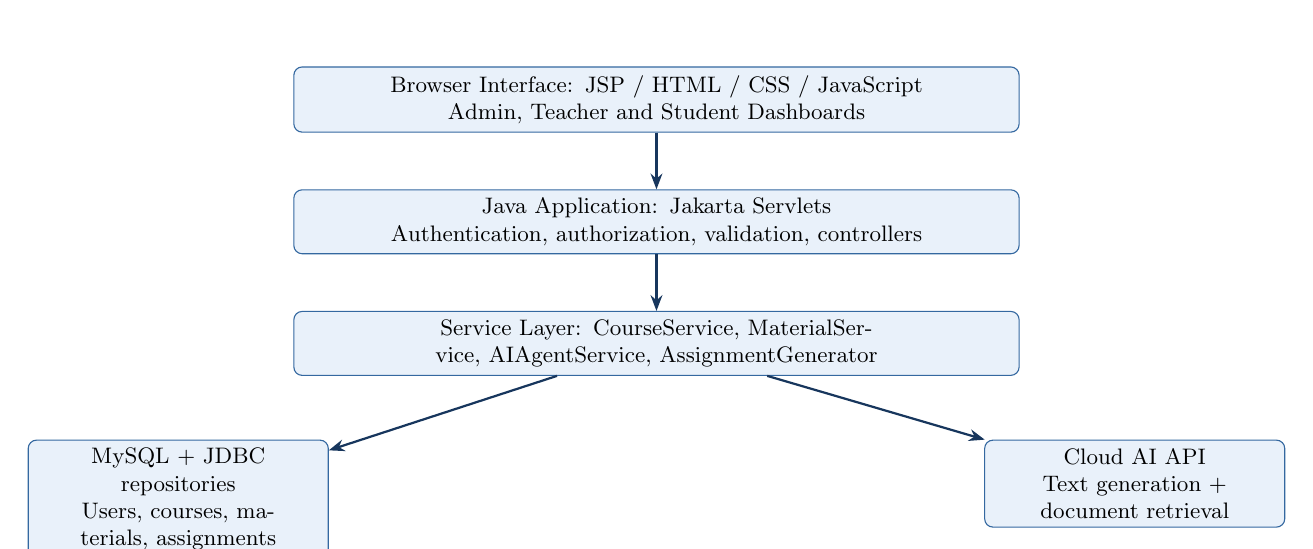
\begin{tikzpicture}[scale=0.90,transform shape,node distance=8mm]
\node[box,text width=10cm] (ui) {Browser Interface: JSP / HTML / CSS / JavaScript\\Admin, Teacher and Student Dashboards};
\node[box,text width=10cm,below=of ui] (serv) {Java Application: Jakarta Servlets\\Authentication, authorization, validation, controllers};
\node[box,text width=10cm,below=of serv] (logic) {Service Layer: CourseService, MaterialService, AIAgentService, AssignmentGenerator};
\node[box,text width=4.0cm,below left=9mm and -5mm of logic] (db) {MySQL + JDBC repositories\\Users, courses, materials, assignments};
\node[box,text width=4.0cm,below right=9mm and -5mm of logic] (ai) {Cloud AI API\\Text generation + document retrieval};
\draw[arrow] (ui)--(serv);\draw[arrow] (serv)--(logic);\draw[arrow] (logic)--(db);\draw[arrow] (logic)--(ai);
\end{tikzpicture}\end{adjustbox}\end{center}
The application will be built using Java, Jakarta Servlet API, JSP, JDBC, MySQL, Maven and Apache Tomcat. The AI integration can use the official OpenAI Java SDK and Responses API; hosted file search is a candidate retrieval option. Alternatively, the Java service can extract document text and retrieve approved excerpts locally before sending only those excerpts to the API. The implementation decision will be validated during the AI integration milestone.
\section{AI Academic Agent: Design and Governance}
\heading{Student workflow.} After confirming course enrollment, the service identifies the selected document or permitted course collection, retrieves relevant content, sends a constrained prompt to the cloud API, and returns a summary or answer with document attribution. When evidence is insufficient, the assistant must state that the available material does not support the answer.
\heading{Teacher workflow.} A teacher selects a course, topic/material, question format, number of questions, difficulty and marks. The AI drafts questions and an optional marking rubric. The draft is stored separately from published assignments. The teacher can edit, discard or approve it; publishing requires an explicit teacher action.
\heading{Safeguards.} Apply authorization before retrieval; never allow model output to override server permissions; do not send passwords or unnecessary student identifiers; label AI-generated content; treat uploaded documents as untrusted text; provide rate limiting, auditing and teacher oversight. The system must not expose unpublished assignment answers to students.
\section{Software Process Model}
\textbf{Selected model: Iterative and Incremental Development.} The first increment establishes the database and authenticated roles; the second implements academic administration; the third adds material management and AI assistance; the fourth focuses on testing, refinement, and documentation. This model fits a capstone because each increment produces demonstrable functionality while allowing feedback and controlled revisions.
\section{Schedule, Milestones and Deliverables}
The following eight-week plan is a \emph{proposed} schedule, to be aligned with the actual course calendar; it does not imply work was completed before the assignment deadline.
\begin{center}\begin{tabular}{p{0.57\textwidth}p{0.29\textwidth}}\toprule Work package&Scheduled weeks\\\midrule
Requirements and feasibility&W1\\
Proposal and process plan&W1--W2\\
Diagrams and schema&W2--W3\\
Java/Maven foundation&W3\\
Core academic modules&W4--W5\\
AI material and assignment tools&W5--W6\\
Testing and correction&W7\\
Documentation and submission&W8\\
\bottomrule\end{tabular}\end{center}
\begin{center}
\begin{adjustbox}{max width=\linewidth}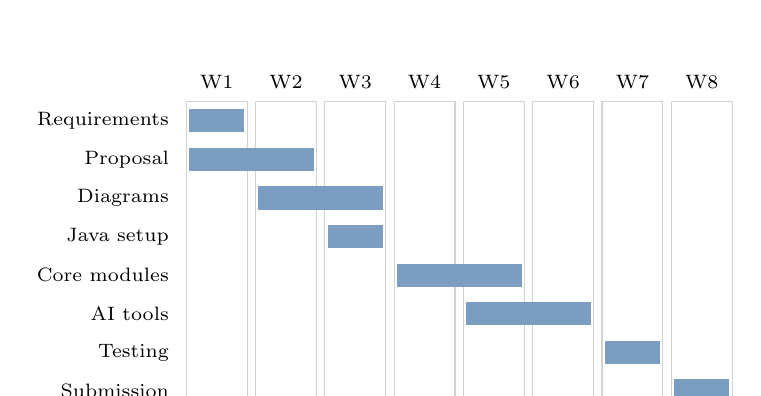
\begin{tikzpicture}[x=0.88cm,y=0.49cm,font=\scriptsize]
\foreach \w in {1,...,8} {\node at (\w,0) {W\w}; \draw[gray!35] (\w-0.44,-8.4) rectangle (\w+0.44,-0.5);}
\foreach \r/\label in {1/Requirements,2/Proposal,3/Diagrams,4/Java setup,5/Core modules,6/AI tools,7/Testing,8/Submission} {\node[anchor=east] at (0.45,-\r) {\label};}
\foreach \r/\a/\b in {1/1/1,2/1/2,3/2/3,4/3/3,5/4/5,6/5/6,7/7/7,8/8/8} {\fill[blue!65] (\a-0.40,-\r-0.30) rectangle (\b+0.40,-\r+0.30);}
\end{tikzpicture}\end{adjustbox}
\end{center}
\begin{tabular}{p{0.16\textwidth}p{0.2\textwidth}p{0.56\textwidth}}\toprule Milestone&Target&Verifiable deliverable\\\midrule M1&End W2&Proposal, requirements baseline, process model\\M2&End W3&Six diagrams, relational schema, Maven skeleton\\M3&End W5&Role-based CRUD prototype with five or more Java classes\\M4&End W6&Material-grounded Q\&A and teacher assignment draft demo\\M5&End W8&Test report, screenshots, README, GitHub repository\\\bottomrule\end{tabular}
\section{Data Flow Diagram (Level 0 / Context)}
\begin{center}
\begin{adjustbox}{max width=\linewidth}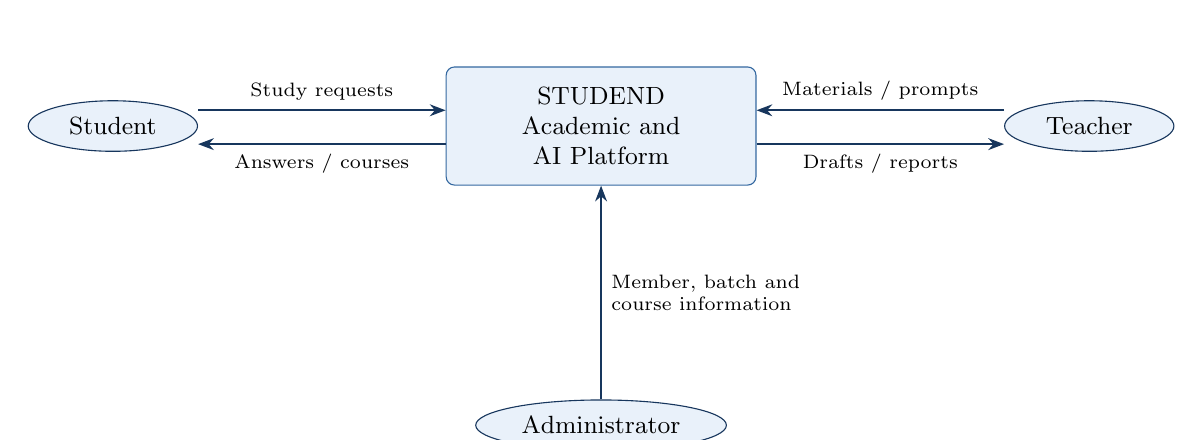
\begin{tikzpicture}[x=1cm,y=1cm,>=Stealth,font=\scriptsize]
\node[actor,minimum width=2.15cm] (student) at (0,1.45) {Student};
\node[actor,minimum width=2.15cm] (teacher) at (12.4,1.45) {Teacher};
\node[actor,minimum width=2.15cm] (admin) at (6.2,-2.35) {Administrator};
\node[box,text width=3.7cm,minimum height=1.5cm] (system) at (6.2,1.45) {STUDEND\\Academic and AI Platform};
\draw[arrow] (student.east) ++(0,0.20) -- node[above]{Study requests} ([yshift=0.20cm]system.west);
\draw[arrow] ([yshift=-0.23cm]system.west) -- node[below]{Answers / courses} ([yshift=-0.23cm]student.east);
\draw[arrow] ([yshift=0.20cm]teacher.west) -- node[above]{Materials / prompts} ([yshift=0.20cm]system.east);
\draw[arrow] ([yshift=-0.23cm]system.east) -- node[below]{Drafts / reports} ([yshift=-0.23cm]teacher.west);
\draw[arrow] (admin.north) -- node[right,align=left]{Member, batch and\\course information} (system.south);
\end{tikzpicture}\end{adjustbox}
\end{center}
\section{Use Case Diagram}
\begin{center}\begin{adjustbox}{max width=\linewidth}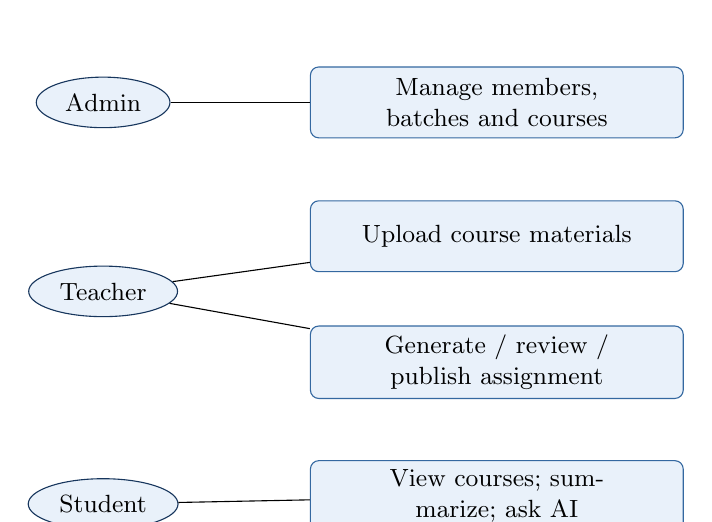
\begin{tikzpicture}[node distance=7mm]
\node[actor] (admin) at (0,3) {Admin};\node[actor] (teacher) at (0,0.6) {Teacher};\node[actor] (student) at (0,-2.1) {Student};
\node[box,text width=4.5cm] (u1) at (5,3) {Manage members, batches and courses};
\node[box,text width=4.5cm] (u2) at (5,1.3) {Upload course materials};
\node[box,text width=4.5cm] (u3) at (5,-0.3) {Generate / review / publish assignment};
\node[box,text width=4.5cm] (u4) at (5,-2.0) {View courses; summarize; ask AI};
\draw (admin)--(u1);\draw (teacher)--(u2);\draw (teacher)--(u3);\draw (student)--(u4);
\end{tikzpicture}\end{adjustbox}\end{center}
\section{Activity Diagram: Teacher AI Assignment}
\begin{center}\begin{adjustbox}{max width=\linewidth}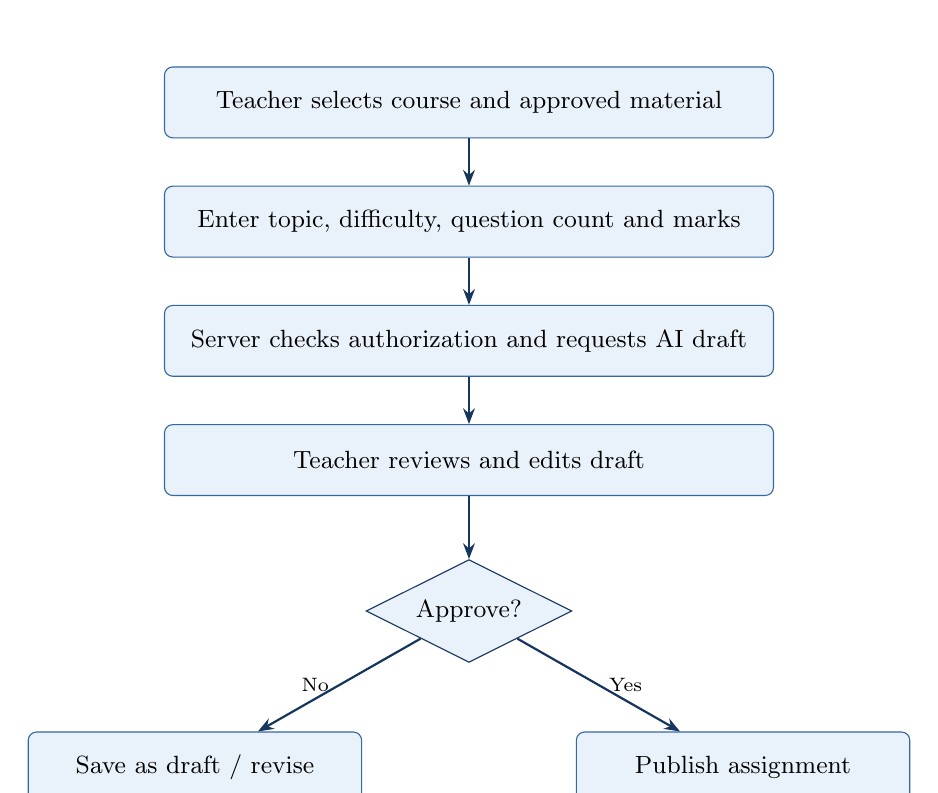
\begin{tikzpicture}[node distance=6mm]
\node[box,text width=7.5cm] (a) {Teacher selects course and approved material};
\node[box,text width=7.5cm,below=of a] (b) {Enter topic, difficulty, question count and marks};
\node[box,text width=7.5cm,below=of b] (c) {Server checks authorization and requests AI draft};
\node[box,text width=7.5cm,below=of c] (d) {Teacher reviews and edits draft};
\node[draw=navy,diamond,aspect=2,fill=pale,below=8mm of d,align=center,font=\small] (e) {Approve?};
\node[box,text width=4cm,below left=12mm and 7mm of e] (f) {Save as draft / revise};
\node[box,text width=4cm,below right=12mm and 7mm of e] (g) {Publish assignment};
\foreach \x/\y in {a/b,b/c,c/d,d/e} \draw[arrow] (\x)--(\y);
\draw[arrow] (e)--node[left,font=\scriptsize]{No}(f);\draw[arrow] (e)--node[right,font=\scriptsize]{Yes}(g);
\end{tikzpicture}\end{adjustbox}\end{center}
\section{Entity Relationship Diagram (Conceptual)}
\begin{center}\begin{adjustbox}{max width=\linewidth}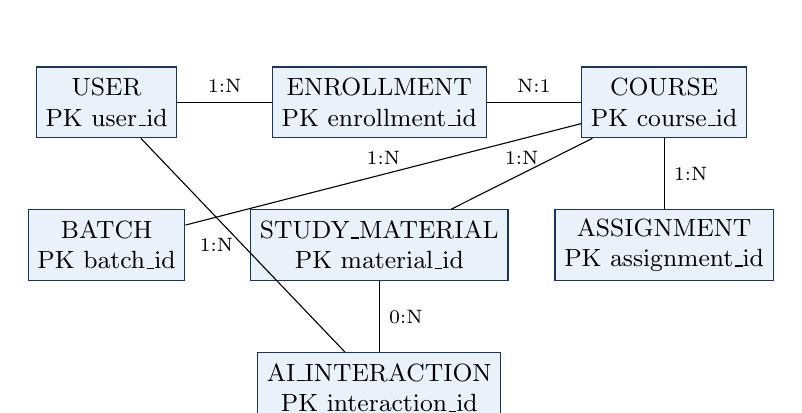
\begin{tikzpicture}[node distance=9mm and 12mm,every node/.style={font=\scriptsize}]
\node[entity] (user) {USER\\PK user\_id};\node[entity,right=of user] (enroll) {ENROLLMENT\\PK enrollment\_id};\node[entity,right=of enroll] (course) {COURSE\\PK course\_id};
\node[entity,below=of user] (batch) {BATCH\\PK batch\_id};\node[entity,below=of enroll] (material) {STUDY\_MATERIAL\\PK material\_id};\node[entity,below=of course] (assign) {ASSIGNMENT\\PK assignment\_id};
\node[entity,below=of material] (chat) {AI\_INTERACTION\\PK interaction\_id};
\draw (user)--node[above]{1:N}(enroll);\draw (enroll)--node[above]{N:1}(course);\draw (batch)--node[above]{1:N}(course);\draw (course)--node[right]{1:N}(assign);\draw (course)--node[above]{1:N}(material);\draw (user)--node[left]{1:N}(chat);\draw (material)--node[right]{0:N}(chat);
\end{tikzpicture}\end{adjustbox}\end{center}
The logical schema will additionally enforce teacher-course assignments, university tenancy and batch membership. The diagram is simplified for proposal readability; cardinalities and keys will be refined during database design.
\section{Class Diagram (Initial Domain and Service Model)}
\begin{center}
\begin{adjustbox}{max width=\linewidth}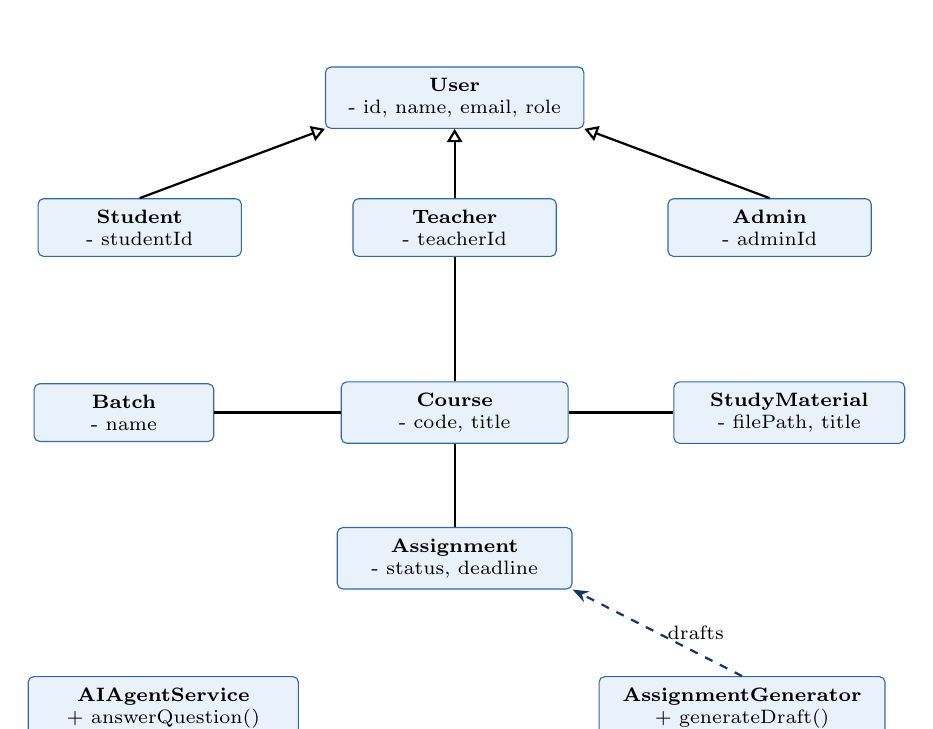
\begin{tikzpicture}[x=1cm,y=1cm,font=\scriptsize,>=Stealth]
\tikzset{cls/.style={draw=blue,fill=pale,rounded corners=2pt,align=center,minimum height=0.65cm,inner sep=4pt}}
\node[cls,text width=3.0cm] (user) at (6.2,0) {\textbf{User}\\- id, name, email, role};
\node[cls,text width=2.3cm] (student) at (2.2,-1.65) {\textbf{Student}\\- studentId};
\node[cls,text width=2.3cm] (teacher) at (6.2,-1.65) {\textbf{Teacher}\\- teacherId};
\node[cls,text width=2.3cm] (admin) at (10.2,-1.65) {\textbf{Admin}\\- adminId};
\draw[-{Triangle[open]},thick] (student.north) -- (user.south west);
\draw[-{Triangle[open]},thick] (teacher.north) -- (user.south);
\draw[-{Triangle[open]},thick] (admin.north) -- (user.south east);
\node[cls,text width=2.0cm] (batch) at (2.0,-4.0) {\textbf{Batch}\\- name};
\node[cls,text width=2.6cm] (course) at (6.2,-4.0) {\textbf{Course}\\- code, title};
\node[cls,text width=2.65cm] (material) at (10.45,-4.0) {\textbf{StudyMaterial}\\- filePath, title};
\draw[thick] (teacher.south) -- (course.north);
\draw[thick] (batch.east) -- (course.west);
\draw[thick] (course.east) -- (material.west);
\node[cls,text width=2.7cm] (assignment) at (6.2,-5.85) {\textbf{Assignment}\\- status, deadline};
\draw[thick] (course.south) -- (assignment.north);
\node[cls,text width=3.15cm] (agent) at (2.5,-7.75) {\textbf{AIAgentService}\\+ answerQuestion()};
\node[cls,text width=3.35cm] (generator) at (9.85,-7.75) {\textbf{AssignmentGenerator}\\+ generateDraft()};

\draw[arrow,dashed] (generator.north) -- node[right]{drafts} (assignment.south east);
\end{tikzpicture}\end{adjustbox}
\end{center}
The prototype will implement at least \texttt{User}, \texttt{Student}, \texttt{Teacher}, \texttt{Batch}, \texttt{Course}, \texttt{StudyMaterial}, and \texttt{Assignment}, supported by servlet controllers and JDBC repositories. The inheritance and associations shown are conceptual and will be checked against the implementation.
\section{Object Diagram (Illustrative Snapshot)}
\begin{center}
\begin{adjustbox}{max width=\linewidth}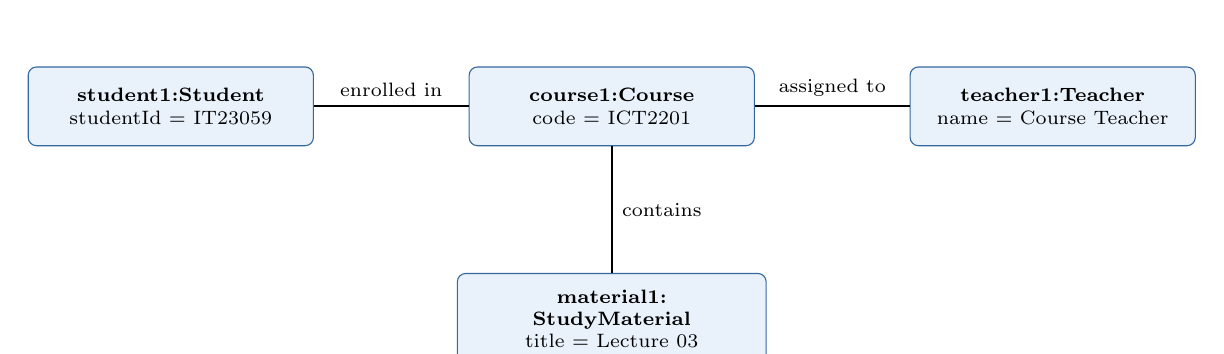
\begin{tikzpicture}[x=1cm,y=1cm,font=\scriptsize,>=Stealth]
\tikzset{obj/.style={draw=blue,fill=pale,rounded corners=3pt,align=center,minimum height=1.0cm,inner sep=6pt}}
\node[obj,text width=3.2cm] (student) at (0,0) {\textbf{student1:Student}\\studentId = IT23059};
\node[obj,text width=3.2cm] (course) at (5.6,0) {\textbf{course1:Course}\\code = ICT2201};
\node[obj,text width=3.2cm] (teacher) at (11.2,0) {\textbf{teacher1:Teacher}\\name = Course Teacher};
\node[obj,text width=3.5cm] (material) at (5.6,-2.7) {\textbf{material1:}\\\textbf{StudyMaterial}\\title = Lecture 03};
\draw[thick] (student.east) -- node[above]{enrolled in} (course.west);
\draw[thick] (course.east) -- node[above]{assigned to} (teacher.west);
\draw[thick] (course.south) -- node[right]{contains} (material.north);
\end{tikzpicture}\end{adjustbox}
\end{center}
These objects are sample instances for the diagram and do not represent verified production records.
\section{Prototype Interface and Demonstration}
\begin{tabular}{p{0.29\textwidth}p{0.63\textwidth}}\toprule Page&Demonstrated interactions\\\midrule Login / role routing&Authenticate and display role-specific dashboard\\Admin dashboard&Create/list students, teachers, batches and courses\\Teacher course page&Upload material; request AI assignment draft; edit and publish\\Student course page&View assigned material; request summary; ask a question\\AI response view&Display answer, source reference, warning when insufficient evidence\\\bottomrule\end{tabular}
\section{Feasibility, Risks and Mitigations}
\begin{longtable}{p{0.28\textwidth}p{0.64\textwidth}}\toprule Risk or constraint&Mitigation\\\midrule\endhead
API cost and connectivity&Request quotas, model configuration, retry policy, clear fallback UI\\Hallucinated AI content&Material-grounded retrieval, citations, uncertainty disclosure, human review\\Data privacy&Authorization checks, data minimization, institution-approved uploads, retention controls\\Unauthorized course access&Enforce membership checks server-side for every file and AI request\\Malicious or oversized files&Allowed file types, size limits, safe storage, content validation\\Time and scope overrun&Incremental milestones; prioritize five-class working prototype\\Database inconsistencies&Foreign keys, constraints, transactions and test fixtures\\\bottomrule\end{longtable}
\section{Testing and Evaluation Plan}
Unit tests will validate entities and business rules; integration tests will verify JDBC persistence, servlet authorization, and course assignment; functional tests will exercise each role's main workflow; negative tests will attempt unauthorized material access. For AI, a curated set of questions will be compared with lecture content, checking factual grounding, attribution, and appropriate abstention. Teacher-generated assignments will be evaluated for topic relevance, clarity, marks allocation, and whether approval is required before publication. No quantitative accuracy claims will be made until testing is completed.
\section{Estimated Resources and Budget}
Development tools (JDK, Maven, MySQL community tools, Git) can be used without software licensing fees under their respective terms. The prototype requires a development computer, a Tomcat server, database storage, network access for AI calls, and an API account. Cloud API and hosting charges are variable and will be measured rather than assumed; a fixed request quota will be used during the demonstration.
\section{Deliverables and GitHub Submission}
\begin{enumerate}[leftmargin=*]\item Final LaTeX proposal and compiled PDF.\item Six required diagrams and editable diagram sources.\item Maven Java source code, JSP/CSS/JS assets, and database setup scripts.\item Screenshots of the prototype and test results.\item README with architecture, prerequisites, build/run instructions, feature status, and limitations.\item Public GitHub repository URL submitted through the assignment portal.\end{enumerate}

\clearpage
\section{Background, Rationale and Research Questions}
\subsection{Institutional context}
A typical university course involves several interconnected records: students belong to batches, teachers are assigned to course offerings, and learning resources and assessments must be available to the correct participants. When these records are maintained separately, staff must reconcile conflicting versions and students may struggle to locate authoritative material. STUDEND treats the course offering as the central unit connecting people, content, and learning activities.
\subsection{Research and design questions}
The project will investigate three practical questions: (1) Can a role-aware Java web application reduce repeated administrative operations in a representative course-management workflow? (2) Can retrieval of approved study materials improve the relevance and traceability of AI-generated study answers? (3) Can a human-in-the-loop workflow make AI-generated assignment drafts useful without giving the AI authority to publish assessments?
\subsection{Project contribution}
The proposed contribution is an integrated prototype rather than a new foundation model. Its distinctive feature is the combination of academic permissions, course-specific retrieval, and teacher-controlled AI drafting within a conventional Java enterprise-style architecture.

\section{Detailed User Stories and Acceptance Scenarios}
\begin{longtable}{p{0.10\textwidth}p{0.38\textwidth}p{0.43\textwidth}}
\toprule ID & User story & Acceptance evidence \\\midrule\endhead
US-01 & As an administrator, I want to register a student so the student can access assigned courses. & Valid data creates a membership; duplicate active email is rejected with an explanation.\\
US-02 & As an administrator, I want to assign a teacher and batch to a course. & The course appears in the assigned teacher and enrolled students' dashboards.\\
US-03 & As a teacher, I want to upload lecture notes for my course. & A permitted file is stored, indexed or extracted, and visible only to authorized users.\\
US-04 & As a student, I want to summarize a lecture. & A concise summary is returned and identifies the source material used.\\
US-05 & As a student, I want to ask a question about lecture content. & The answer uses retrieved material and admits when evidence is missing.\\
US-06 & As a teacher, I want AI to propose assignment questions. & The draft reflects specified topic, type, difficulty and marks, and remains unpublished.\\
US-07 & As a teacher, I want to edit and publish a draft. & Only an authorized teacher can publish, and publication is logged.\\
US-08 & As a student, I want my course resources protected. & Requests for a course in which I am not enrolled are denied.\\
\bottomrule
\end{longtable}
\heading{Scenario A: Student learning assistance.} A student logs in, opens an enrolled course, selects an uploaded lecture, and requests an explanation of a topic. The application checks enrollment before retrieving text. The response shows a useful explanation, identifies the material consulted, and marks any unsupported claim as uncertain. If no content is available, the interface explains the limitation instead of fabricating a source.
\heading{Scenario B: Teacher assignment drafting.} A teacher opens an assigned course, chooses a source lecture, requests five short-answer questions with a specified total mark, and reviews the proposed questions and rubric. The draft is saved with a \emph{draft} status. Students cannot see it until the teacher explicitly publishes it.

\section{Data Model and Database Design Decisions}
\subsection{Core entities}
The relational schema will separate identity, institutional membership, course enrollment, teaching resources, and AI activities. This separation reduces duplication and makes authorization checks explicit.
\begin{longtable}{p{0.23\textwidth}p{0.68\textwidth}}
\toprule Entity & Important attributes and purpose\\\midrule\endhead
User & user\_id (PK), name, email (unique), password\_hash, account\_status; global login identity.\\
University & university\_id (PK), name, active\_status; owning institution.\\
Membership & membership\_id (PK), user\_id (FK), university\_id (FK), role, status; institutional access.\\
Batch & batch\_id (PK), university\_id (FK), name; student grouping.\\
BatchMember & batch\_id (FK), membership\_id (FK), joined\_at; many-to-many membership.\\
Course & course\_id (PK), university\_id (FK), code, title, teacher\_membership\_id (FK), batch\_id (FK), status.\\
StudyMaterial & material\_id (PK), course\_id (FK), uploader\_id (FK), title, storage\_path, file\_type, status.\\
MaterialChunk & chunk\_id (PK), material\_id (FK), chunk\_index, extracted\_text, source\_locator; retrievable passages.\\
Assignment & assignment\_id (PK), course\_id (FK), creator\_id (FK), title, status, published\_at.\\
Question & question\_id (PK), assignment\_id (FK), prompt, marks, type, sequence.\\
AIInteraction & interaction\_id (PK), requester\_id (FK), course\_id (FK), purpose, created\_at, outcome; minimal audit metadata.\\
\bottomrule
\end{longtable}
\subsection{Integrity constraints}
Foreign keys will prevent references to nonexistent courses or users. Enrollment uniqueness will be enforced for each batch-member pair. Every repository query for course content will be scoped to the authenticated university and course. Soft deactivation is preferable for memberships and published academic records; destructive deletion requires explicit handling of dependent rows and should not be the default.
\subsection{Illustrative SQL schema fragment}
\begin{verbatim}
CREATE TABLE study_material (
  material_id BIGINT PRIMARY KEY AUTO_INCREMENT,
  course_id BIGINT NOT NULL,
  uploader_id BIGINT NOT NULL,
  title VARCHAR(255) NOT NULL,
  storage_path VARCHAR(500) NOT NULL,
  processing_status VARCHAR(30) NOT NULL,
  FOREIGN KEY (course_id) REFERENCES course(course_id)
);
\end{verbatim}
This fragment illustrates the intended design and is not a claim that the complete database schema has already been executed.

\section{Java Software Architecture and Class Responsibilities}
\subsection{Layered package organization}
\begin{verbatim}
src/main/java/com/studend/
  model/       User, Student, Teacher, Batch, Course, Assignment
  repository/  UserRepository, CourseRepository, MaterialRepository
  service/     AuthService, CourseService, MaterialService
               AIAgentService, AssignmentGenerator
  servlet/     LoginServlet, CourseServlet, AIChatServlet
               AssignmentServlet, MaterialUploadServlet
  security/    AuthorizationFilter, SessionUtil
src/main/webapp/WEB-INF/views/
  login.jsp, admin-dashboard.jsp, teacher-dashboard.jsp
  student-dashboard.jsp, ai-chat.jsp, assignment-editor.jsp
\end{verbatim}
\subsection{Object-oriented design}
The prototype will include more than five Java domain classes, including \texttt{User}, \texttt{Student}, \texttt{Teacher}, \texttt{Batch}, \texttt{Course}, \texttt{StudyMaterial}, and \texttt{Assignment}. The application will use encapsulation for entity state, interfaces for repository abstractions, and composition between services and repositories. Student and Teacher may specialize User at the conceptual level, while persistence may use a single User table plus role-based memberships. The final class diagram will document whichever mapping is actually implemented.
\subsection{Request lifecycle}
For a normal course-management request, the browser submits an HTTP request to a servlet. The servlet validates input and checks session authorization, delegates to a service, and returns a JSP view or structured response. The service calls a repository using parameterized JDBC statements. For AI requests, the service first checks course access, then calls the retrieval component and cloud model client. The cloud API credential is loaded from server configuration rather than embedded in a JSP or GitHub repository.
\subsection{Illustrative interface contracts}
\begin{verbatim}
interface MaterialRepository {
    List<StudyMaterial> findAccessibleByCourse(long courseId);
    Optional<StudyMaterial> findById(long materialId);
}
interface AcademicAIService {
    StudyAnswer answerQuestion(long userId, long courseId,
                               String question);
    AssignmentDraft generateDraft(long teacherId,
                                  AssignmentRequest request);
}
\end{verbatim}
These interfaces are proposed contracts; implementations and method signatures may evolve during prototyping.

\section{AI Retrieval, Prompting and Human Oversight}
\subsection{Document processing and retrieval}
The initial system will accept a controlled set of text-based PDF and plain-text files. Uploaded files are validated by type and size, stored outside the public web directory, and associated with a course. Extracted text is divided into passages with document identifiers and page or section locators when available. For a student question, the retrieval layer selects relevant passages from authorized materials only. A later increment may use embeddings or a managed file-search service for semantic retrieval.
\subsection{Grounded response generation}
The AI request will contain the student's question, retrieved excerpts, and instructions to answer only from the provided material. The output will distinguish evidence-backed explanations from uncertainty and include document attribution where supported. Prompt instructions do not replace backend access controls; the server must filter sources before sending any text to the model.
\subsection{Assignment generation}
The teacher supplies the course, topic, learning objective, format, difficulty, question count, marks and optional source materials. The model produces a structured draft. The Java service validates the requested number of questions, total marks and response format, then saves it as a draft. A teacher can revise, discard or publish it. The AI must not directly update publication status.
\subsection{Known limitations}
Cloud-generated text can be inaccurate, incomplete, biased or inconsistent. Scanned PDFs may require OCR that is outside the initial prototype. Citations may refer to retrieved sections without proving every sentence. API latency, rate limits, outages and variable fees may affect the demonstration. Evaluation and human review are therefore part of the design, not optional additions.

\section{Security, Privacy and Responsible AI}
\begin{longtable}{p{0.26\textwidth}p{0.62\textwidth}}
\toprule Risk area & Planned control\\\midrule\endhead
Authentication & Store salted password hashes; rotate session identifiers at login; expire inactive sessions.\\
Authorization & Check university membership, course enrollment and teacher ownership in every relevant service method.\\
File uploads & Restrict allowed formats, validate size and MIME type, sanitize display names, store outside public paths.\\
SQL injection & Use prepared statements and strict server-side validation.\\
Cloud API secret & Keep the key in server environment variables or a protected secret store; never commit it to Git.\\
Data minimization & Send only necessary excerpts and question context; avoid student IDs and private grades in prompts.\\
Prompt injection & Treat retrieved documents as data, never as instructions authorizing actions or data access.\\
AI transparency & Label generated drafts, show uncertainty, and require teacher approval before publication.\\
Availability & Use request timeouts, clear fallback errors, basic rate limiting and usage quotas.\\
Auditability & Record actor, action, resource and outcome without unnecessarily storing sensitive prompt content.\\
\bottomrule
\end{longtable}
Before any real institutional deployment, the university must approve its data processing practices, retention policy, cloud provider arrangement and student-facing notices. Prototype demonstrations should use synthetic or explicitly permitted data.

\section{Verification, Validation and Evaluation Methodology}
\subsection{Testing levels}
\textbf{Unit tests} will cover validators, role checks, course assignment rules, and assignment draft state transitions. \textbf{Integration tests} will exercise JDBC repositories against a test database and verify that unauthorized course queries return no records. \textbf{System tests} will follow end-to-end scenarios through the browser. \textbf{User acceptance tests} will ask representative student and teacher users to complete tasks using a checklist.
\subsection{Proposed test cases}
\begin{longtable}{p{0.12\textwidth}p{0.47\textwidth}p{0.32\textwidth}}
\toprule Test & Action & Expected result\\\midrule\endhead
T-01 & Sign in with valid student credentials. & Student dashboard opens.\\
T-02 & Request admin endpoint as a student. & Access denied; no state change.\\
T-03 & Create a course with teacher and batch. & Record persists; correct users see it.\\
T-04 & Upload an unsupported file type. & Upload rejected safely.\\
T-05 & Ask about a document in another course. & No private content is returned.\\
T-06 & Ask a question unsupported by selected notes. & Response states insufficient evidence.\\
T-07 & Generate an assignment draft. & Draft is editable and not student-visible.\\
T-08 & Publish a draft as an unauthorized user. & Request denied.\\
T-09 & Simulate cloud API timeout. & Clear error; application remains usable.\\
\bottomrule
\end{longtable}
\subsection{AI answer evaluation}
A small benchmark will be created from permitted sample lecture notes, with factual questions and a teacher-reviewed answer key. Responses will be scored for factual correctness, relevance to the source, attribution quality, and appropriate abstention when evidence is absent. Assignment drafts will be checked for alignment with the requested topic, clarity, difficulty, mark totals, and editing effort. Results will be reported as measured observations rather than guaranteed accuracy claims.
\subsection{Completion criteria}
The prototype will be considered demonstrable when at least five domain classes participate in working features, key records persist in MySQL, role checks prevent unauthorized access, a student can receive one grounded AI response, and a teacher can review and publish an AI-generated assignment draft. Any unmet criteria will be documented honestly.

\section{Project Management, Dependencies and Risk Register}
\begin{longtable}{p{0.19\textwidth}p{0.12\textwidth}p{0.13\textwidth}p{0.45\textwidth}}
\toprule Risk & Likelihood & Impact & Response\\\midrule\endhead
Scope expansion & High & High & Freeze the minimum prototype; move extras to backlog.\\
Cloud API outage & Medium & Medium & Show fallback error and use recorded, clearly labeled demo examples for UI tests.\\
AI inaccuracy & High & High & Source retrieval, explicit uncertainty and teacher review.\\
Database integration & Medium & High & Implement schema and repository tests early.\\
Document parsing & Medium & Medium & Begin with text PDFs; exclude scans initially.\\
Schedule slippage & Medium & High & Deliver working increments and prioritize critical paths.\\
Sensitive data exposure & Medium & High & Test authorization and minimize cloud-transmitted data.\\
Cost overrun & Medium & Medium & Set request limits, monitor tokens and define a spending ceiling.\\
\bottomrule
\end{longtable}
\heading{Critical dependencies.} Course and membership records must exist before secure material retrieval can be tested. Document extraction must work before grounded AI answers can be evaluated. Draft assignment storage must exist before teacher publication workflows can be demonstrated. These dependencies justify the incremental development order.
\heading{Change management.} New requirements will be recorded in a backlog, assigned a priority, and evaluated against milestone deadlines. Features that do not support minimum acceptance criteria will be deferred rather than destabilizing the prototype.

\section{Deployment, Maintenance and Reproducibility}
The demonstrator will run locally using JDK, Maven, Tomcat 11 and MySQL. The GitHub repository will contain a setup guide, example environment configuration without secrets, database creation scripts, test data instructions, and screenshots. A clean installation should be reproducible by cloning the repository, configuring the database and cloud API key, building with Maven, deploying the WAR to Tomcat, and running documented smoke tests.
\heading{Operations plan.} The design will include database backup procedures, basic error logging, configuration for AI rate limits, and a manual method to disable AI calls without disabling core course management. A later deployment can add HTTPS termination, automated CI, monitoring, and institutional single sign-on.
\heading{Deliverable traceability.} The proposal describes intended features; the repository README will distinguish implemented, partially implemented and planned functionality. Diagram revisions will be committed alongside major architecture changes. Screenshots will be taken from the actual working application, not generated mockups presented as completed software.

\section{Appendix A: Proposed Screens and Navigation}
\begin{longtable}{p{0.25\textwidth}p{0.63\textwidth}}
\toprule Screen & Main elements\\\midrule\endhead
Login & Email, password, role-aware redirect and error messages.\\
Admin dashboard & Overview counts and links to student, teacher, batch and course management.\\
Manage students & Searchable table, add/edit/deactivate forms and validation messages.\\
Manage courses & Course code, title, assigned teacher, batch, status and actions.\\
Teacher course page & Materials list, upload control, assignments list and AI draft generator.\\
Student course page & Published resources, assignments and AI study assistant entry point.\\
AI study assistant & Material selector, question input, answer panel, source labels and limitations notice.\\
Assignment editor & Generated questions, marks, edit controls, save draft and publish confirmation.\\
\bottomrule
\end{longtable}
\section{Appendix B: Requirements-to-Deliverables Traceability}
\begin{longtable}{p{0.16\textwidth}p{0.35\textwidth}p{0.40\textwidth}}
\toprule Requirement group & Implementation artifact & Verification artifact\\\midrule\endhead
FR-01--05 & Auth, memberships, batch and course services & Role/access and CRUD test cases\\
FR-06 & Upload servlet, MaterialService, StudyMaterial & Upload and course access tests\\
FR-07--08 & AIChatServlet, retrieval, AIAgentService & Grounded answer benchmark and denial tests\\
FR-09--10 & AssignmentGenerator, editor, Assignment & Draft, edit and publish workflow tests\\
FR-11--12 & AIInteraction logging and exception handling & Audit record and timeout tests\\
Process model & Iteration plan, milestones, Gantt chart & Weekly deliverable checklist\\
Diagrams & DFD, Use Case, Activity, ER, Class, Object & Diagram-to-code review\\
Submission & GitHub repository and proposal PDF & README, screenshots and setup verification\\
\bottomrule
\end{longtable}

\section{Conclusion}
STUDEND combines conventional academic administration with a course-aware AI assistant to improve access to learning materials and reduce repetitive assignment preparation. A Java Servlet/JSP architecture, MySQL persistence, explicit authorization, and teacher-controlled publication make the proposal feasible as an incremental capstone. The first prototype will demonstrate a coherent subset of the design; later increments will extend functionality after validation.
\section{References}
\begin{enumerate}[leftmargin=*,itemsep=2pt]\sloppy\item OpenAI, \emph{OpenAI Java API Library}, \url{https://developers.openai.com/api/reference/java}.\item OpenAI, \emph{File Search Guide}, \url{https://developers.openai.com/api/docs/guides/tools-file-search}.\item OpenAI, \emph{Responses API}, \url{https://developers.openai.com/api/reference/java/resources/responses/methods/create}.\item Oracle, \emph{Java Platform Documentation}, \url{https://docs.oracle.com/en/java/}.\item Apache Software Foundation, \emph{Apache Tomcat Documentation}, \url{https://tomcat.apache.org/}.\end{enumerate}
\end{document}
